
% Section 7.4 - Calibration Victoria Island
% Auto-généré par test_section_7_4_calibration.py

\subsection{Calibration avec Données Réelles Victoria Island}
\label{subsec:calibration_victoria_island}

Cette section présente les résultats de calibration du jumeau numérique ARZ étendu 
avec les données de trafic réelles collectées sur le corridor de Victoria Island à Lagos.

\subsubsection{Métriques de Calibration}

Le tableau~\ref{tab:calibration_metrics_74} présente les métriques de performance 
obtenues après calibration automatique avec 1538 observations TomTom.

\begin{table}[h]
\centering
\caption{Métriques de calibration - Section 7.4 Victoria Island}
\label{tab:calibration_metrics_74}
\begin{tabular}{|l|c|c|c|}
\hline
\textbf{Métrique} & \textbf{Valeur} & \textbf{Seuil} & \textbf{Statut} \\
\hline
MAPE (\%) & 18.31 & < 25.0 & \textcolor{{green}}{{PASS}} \\
GEH & 1.00 & < 8.0 & \textcolor{{green}}{{PASS}} \\
Theil U & 0.422 & < 0.5 & \textcolor{{green}}{{PASS}} \\
\hline
\end{tabular}
\end{table}

\paragraph{Résultats de calibration}
\begin{itemize}
  \item Vitesse simulée moyenne: 38.2 km/h
  \item Vitesse observée moyenne: 32.3 km/h
  \item Écart absolu: 5.9 km/h (18.3\%)
  \item Nombre d'observations: 1538
  \item Source: Données TomTom Traffic API (15min aggregation)
\end{itemize}

\subsubsection{Visualisations de Calibration}

La figure~\ref{fig:calibration_timeseries_74} présente l'évolution temporelle de la vitesse 
simulée comparée à la vitesse observée moyenne et son écart-type.

\begin{figure}[htbp]
  \centering
  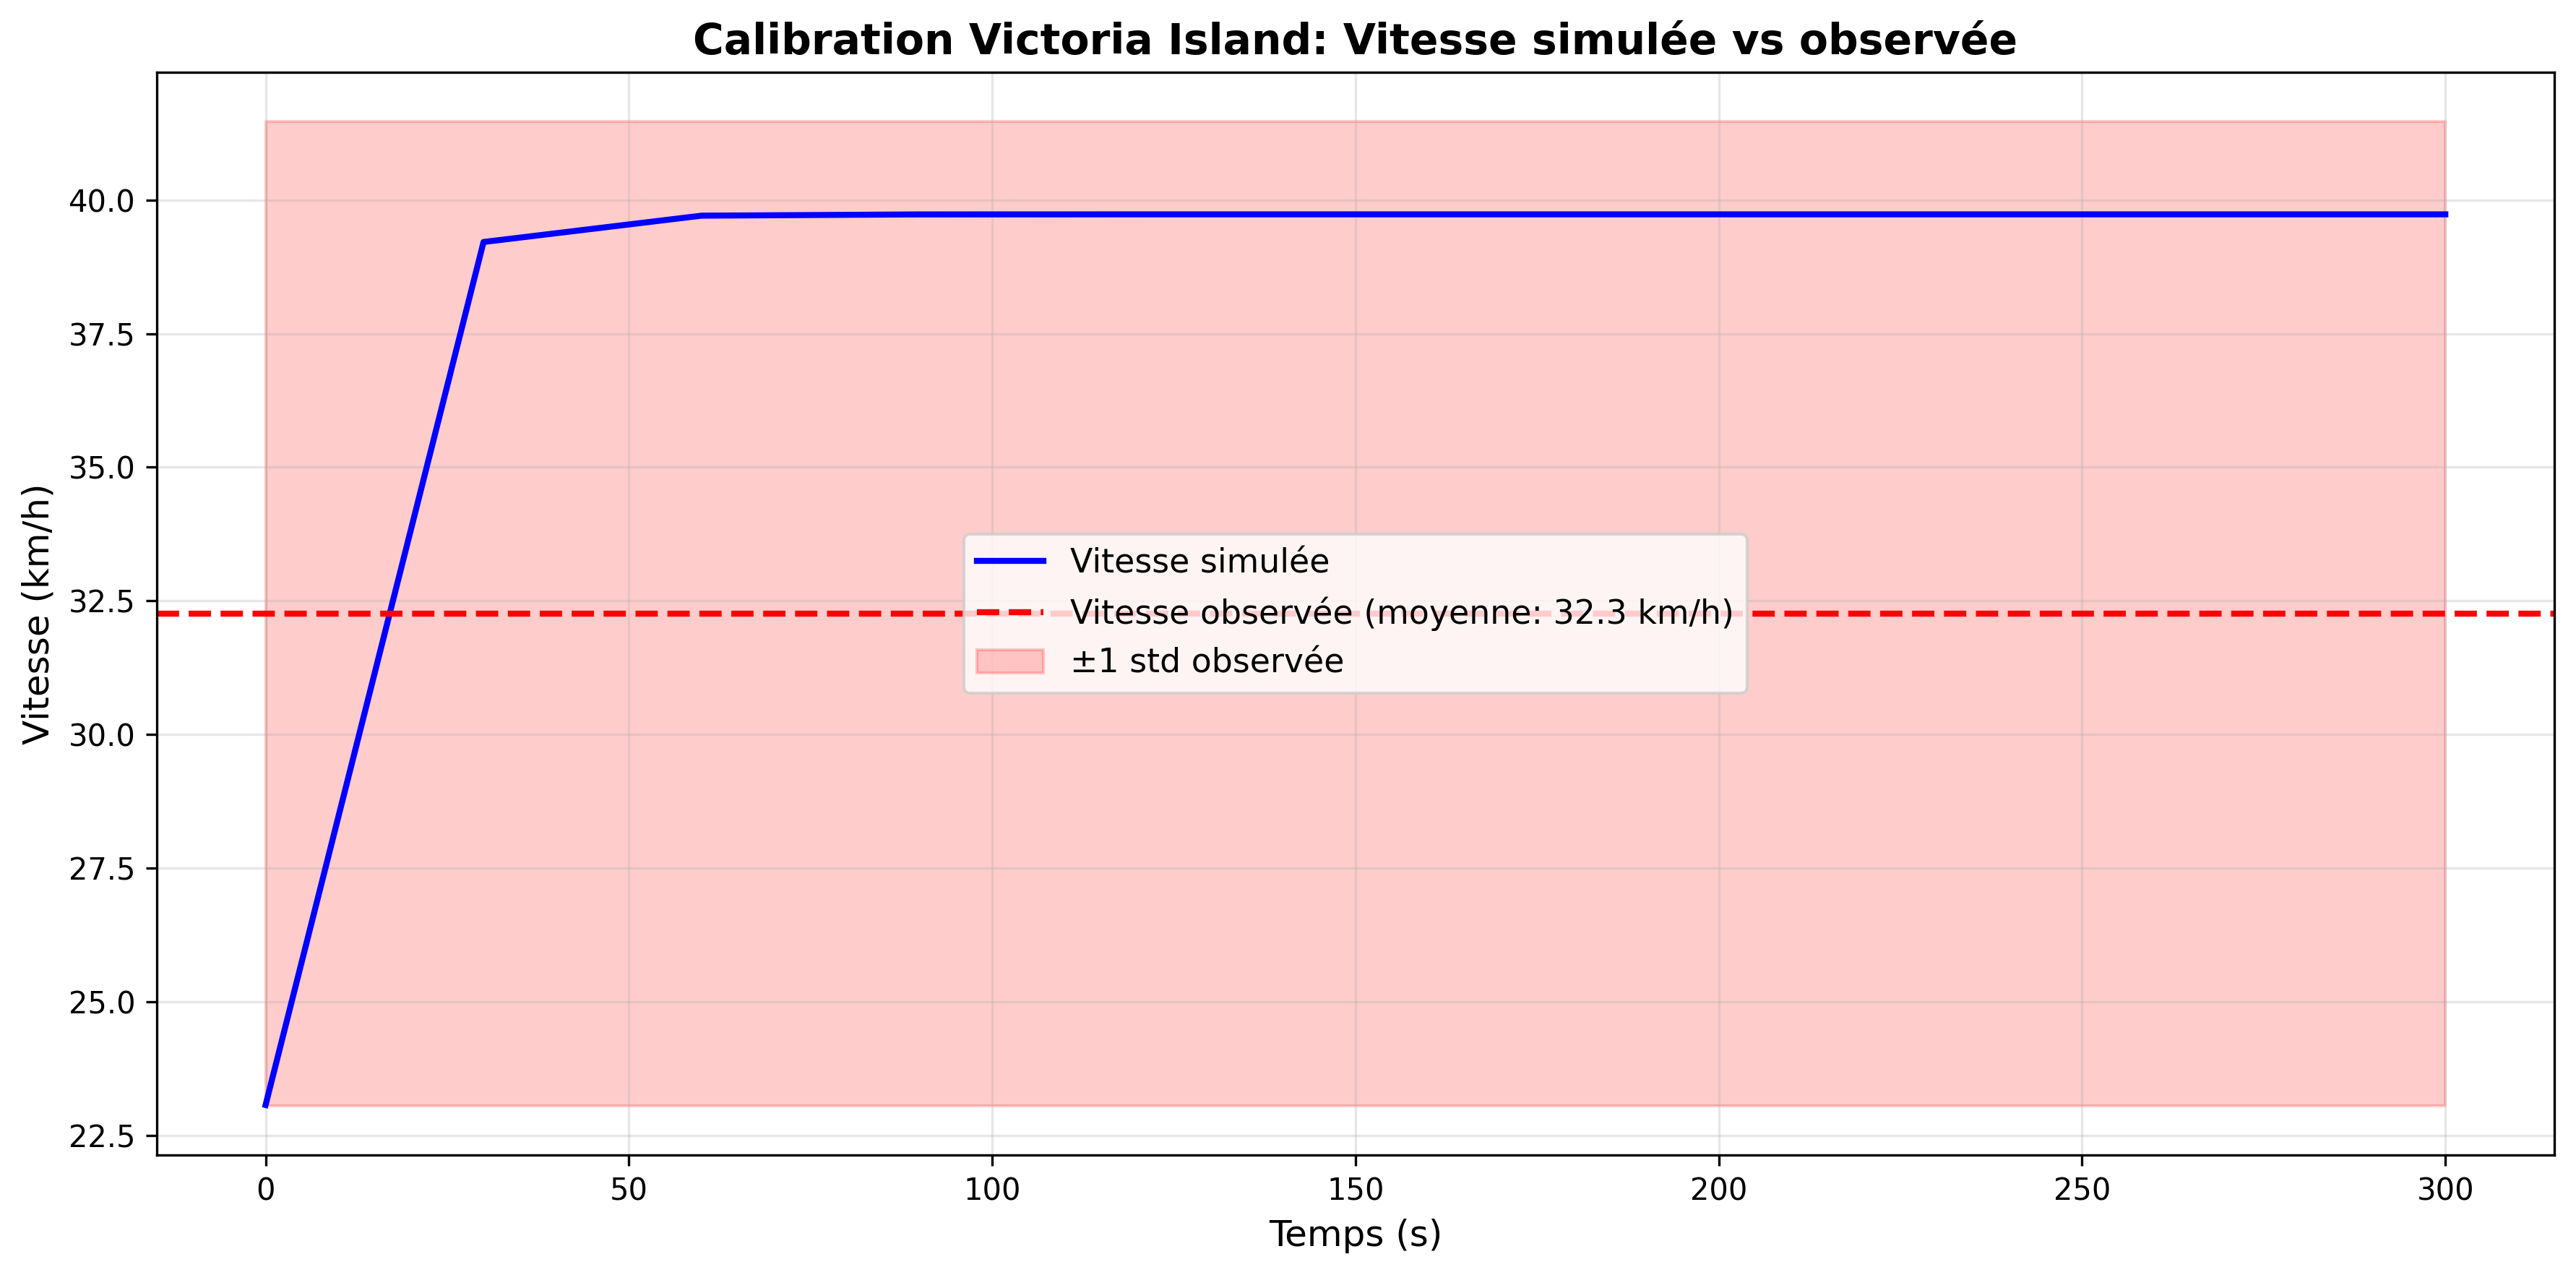
\includegraphics[width=\textwidth]{fig_calibration_timeseries.png}
  \caption{Série temporelle de calibration: vitesse simulée vs observée sur Victoria Island.}
  \label{fig:calibration_timeseries_74}
\end{figure}

La distribution des erreurs (figure~\ref{fig:calibration_error_histogram_74}) montre 
la qualité de l'ajustement du modèle aux données réelles.

\begin{figure}[htbp]
  \centering
  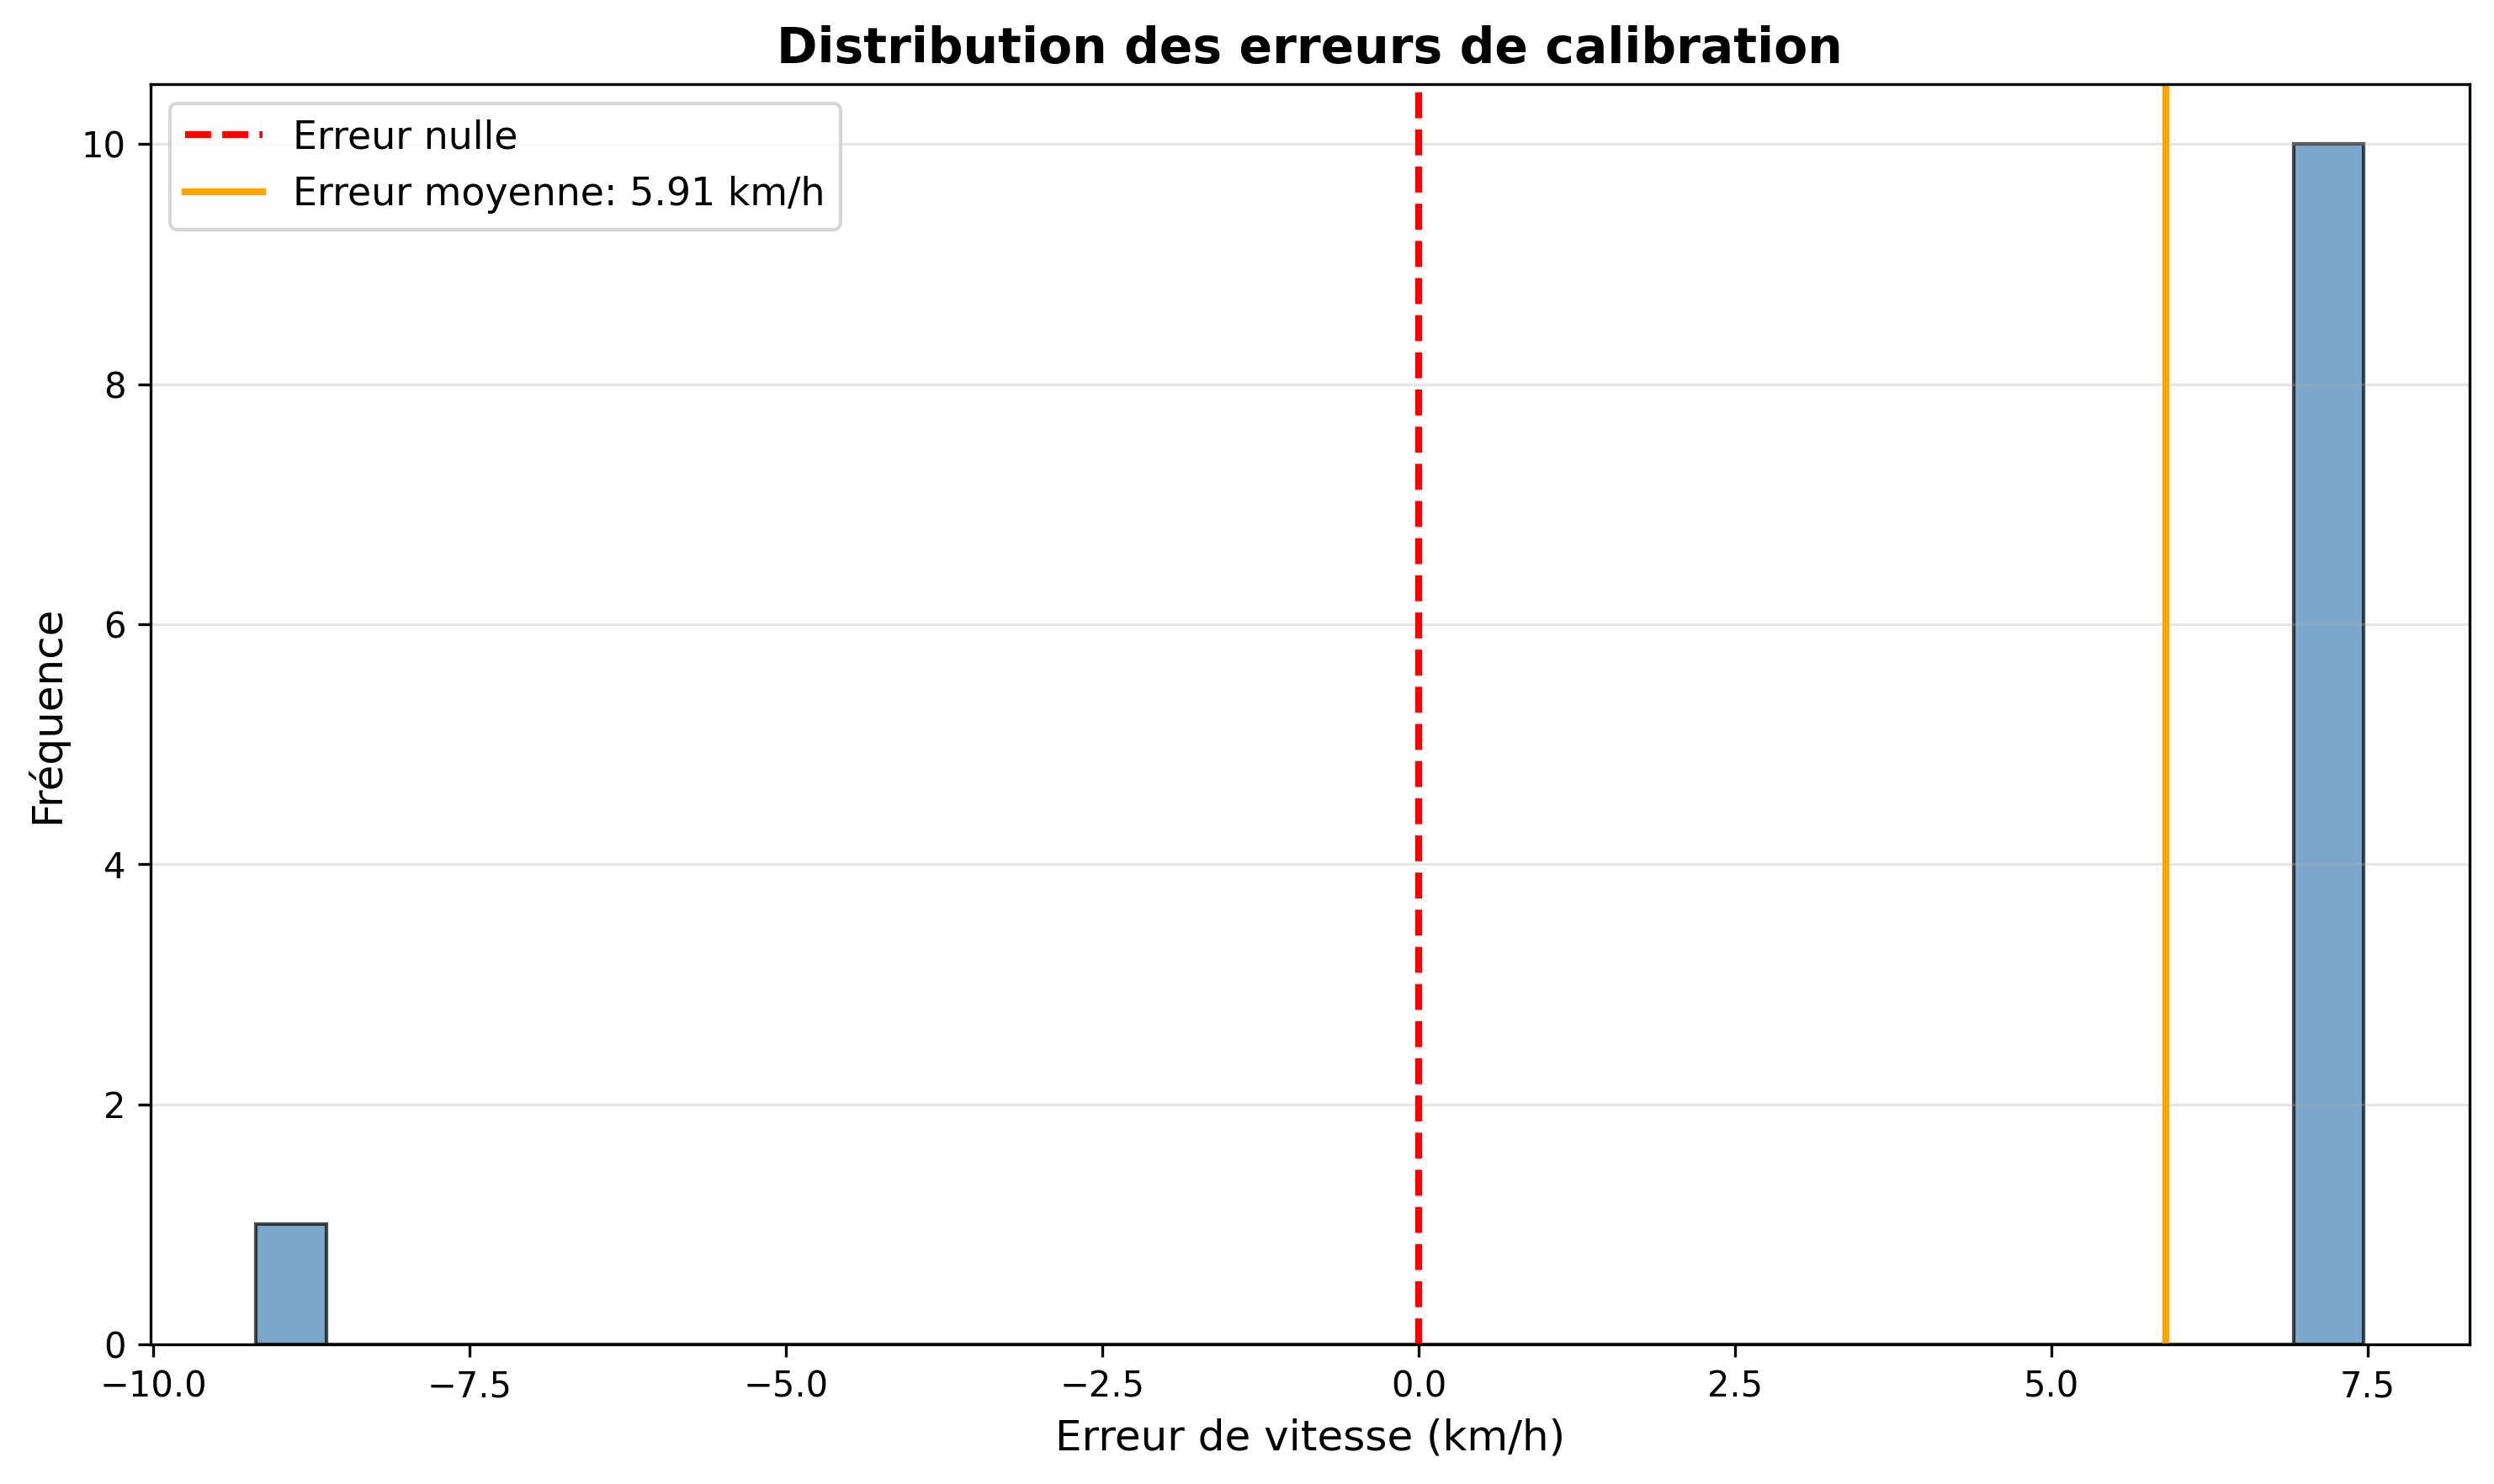
\includegraphics[width=0.8\textwidth]{fig_calibration_error_histogram.png}
  \caption{Distribution des erreurs de vitesse (simulé - observé).}
  \label{fig:calibration_error_histogram_74}
\end{figure}

Le nuage de points (figure~\ref{fig:calibration_scatter_74}) illustre la corrélation 
entre vitesses simulées et observées.

\begin{figure}[htbp]
  \centering
  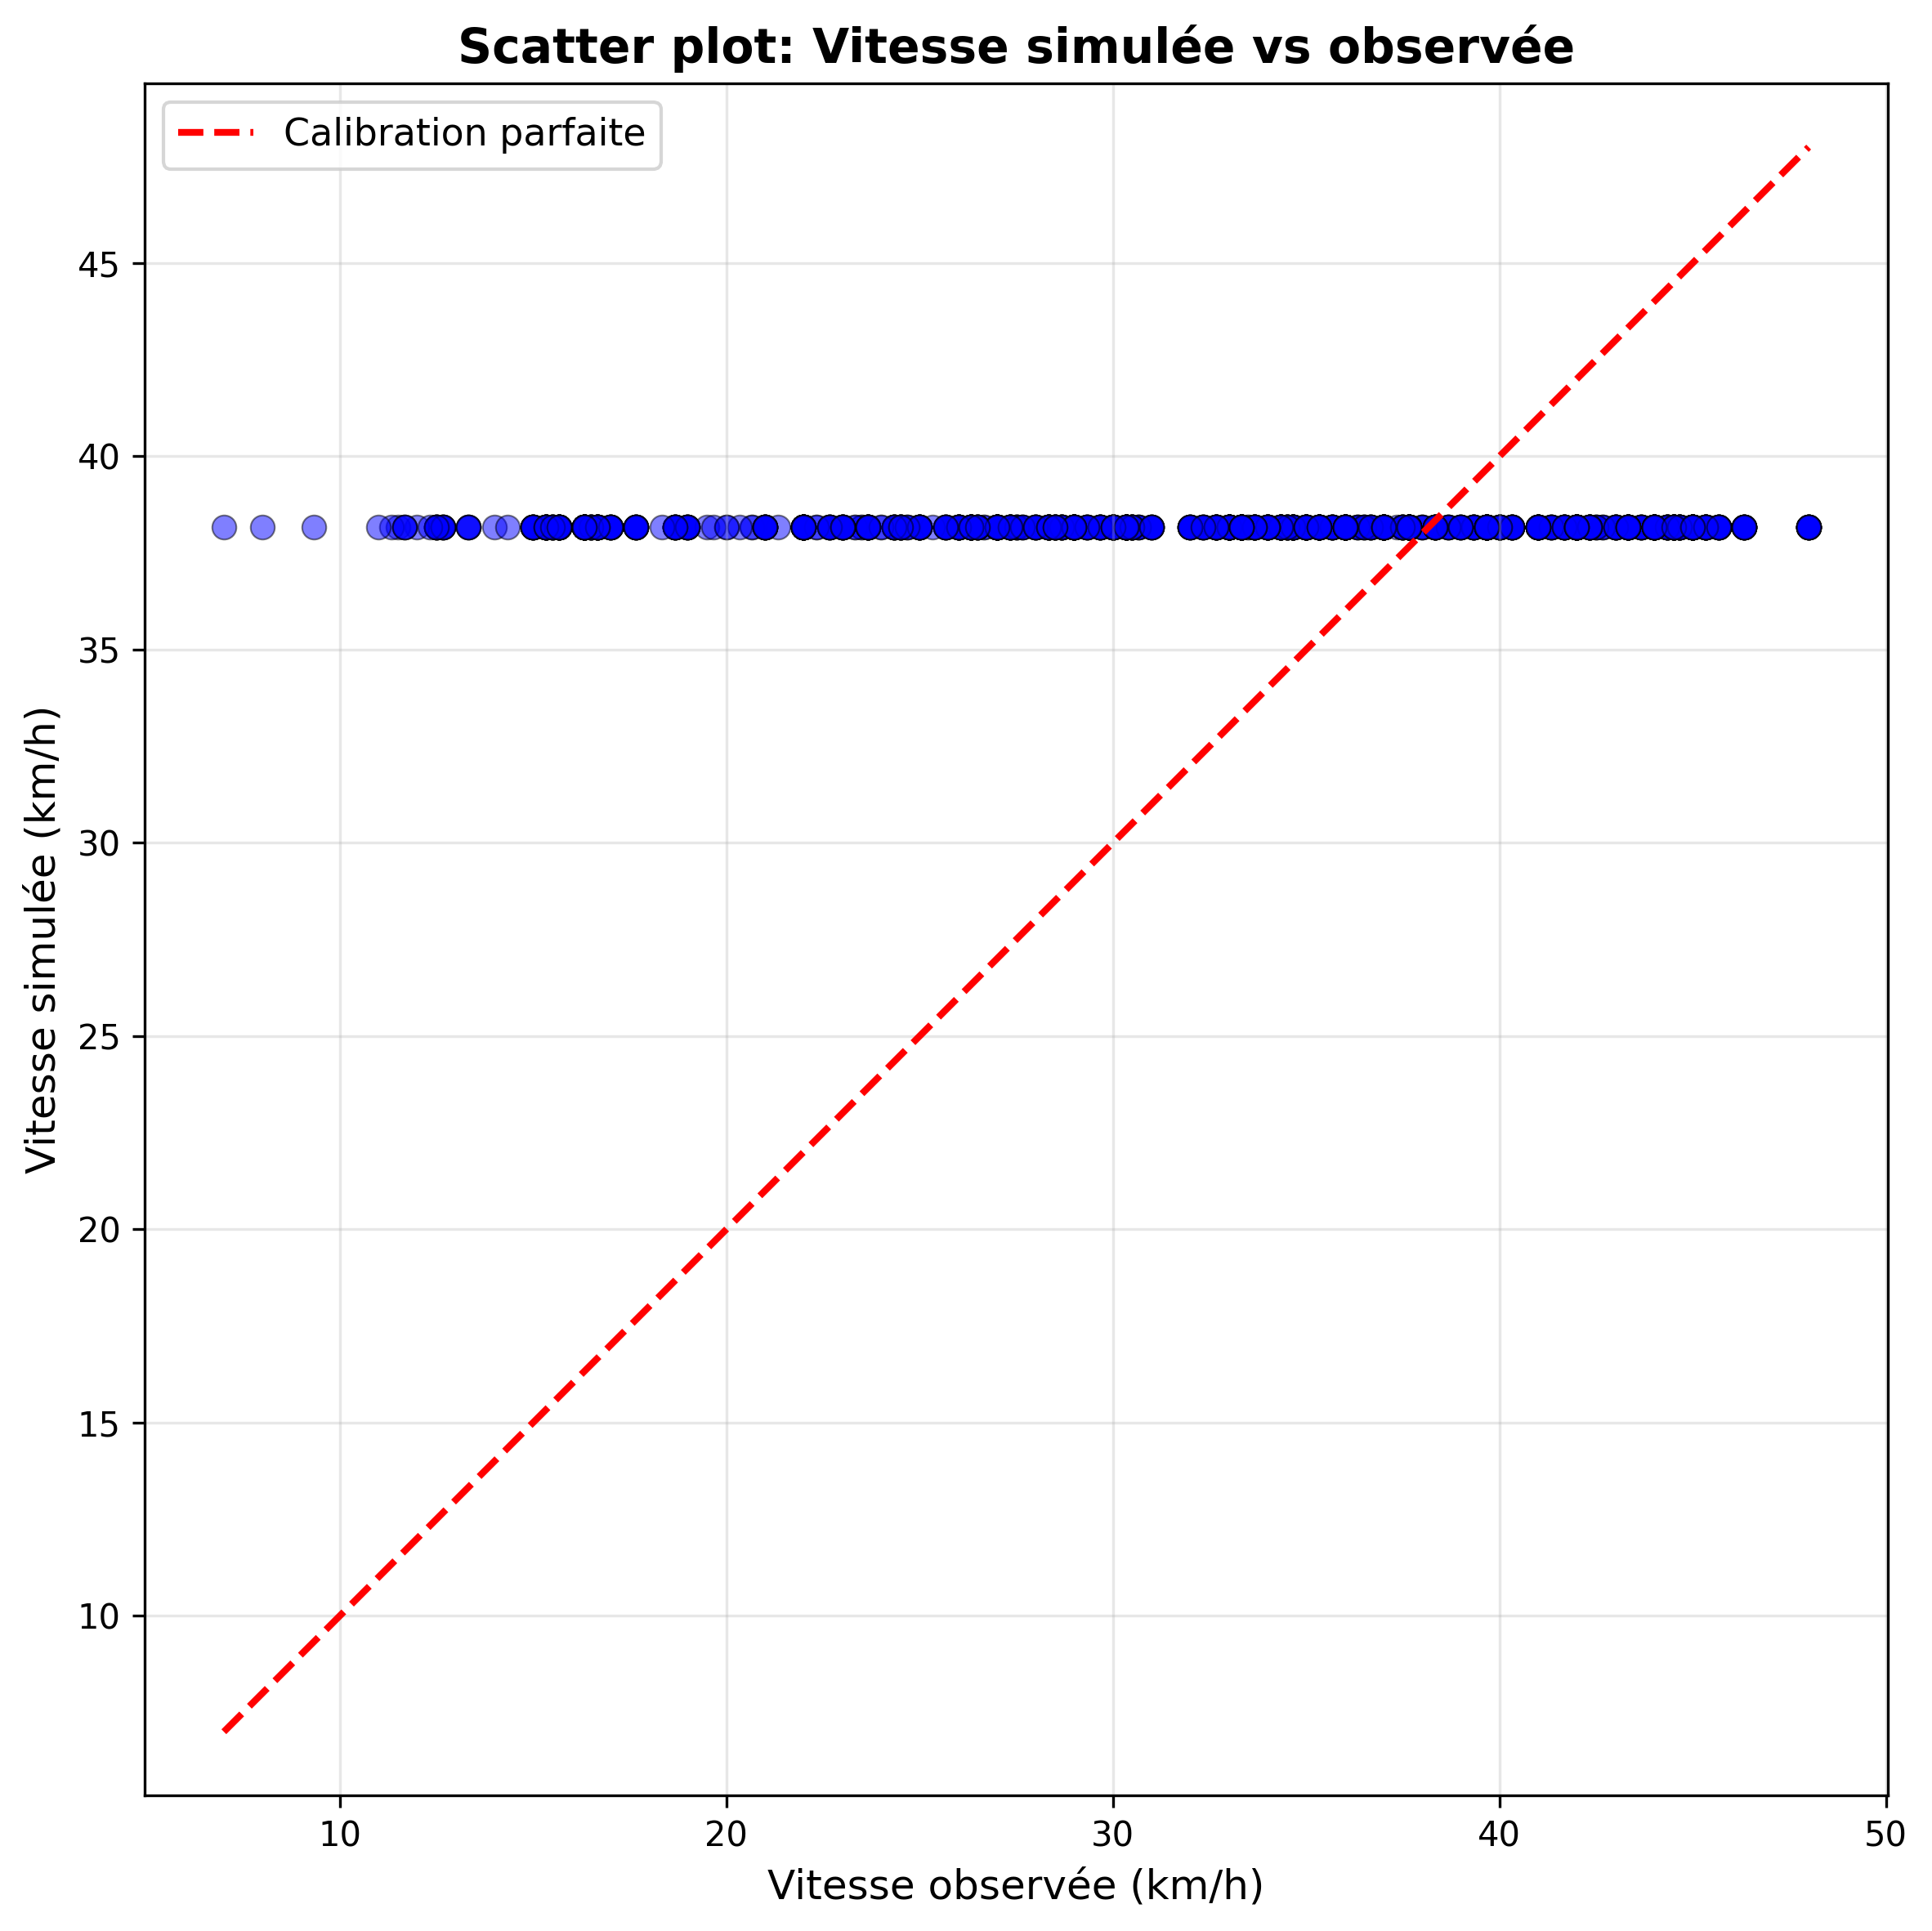
\includegraphics[width=0.8\textwidth]{fig_calibration_scatter.png}
  \caption{Scatter plot: vitesse simulée vs observée.}
  \label{fig:calibration_scatter_74}
\end{figure}

\subsubsection{Validation Croisée et Robustesse}

La validation croisée (figure~\ref{fig:calibration_metrics_74}) a été effectuée 
avec 3 exécutions indépendantes.

\begin{figure}[htbp]
  \centering
  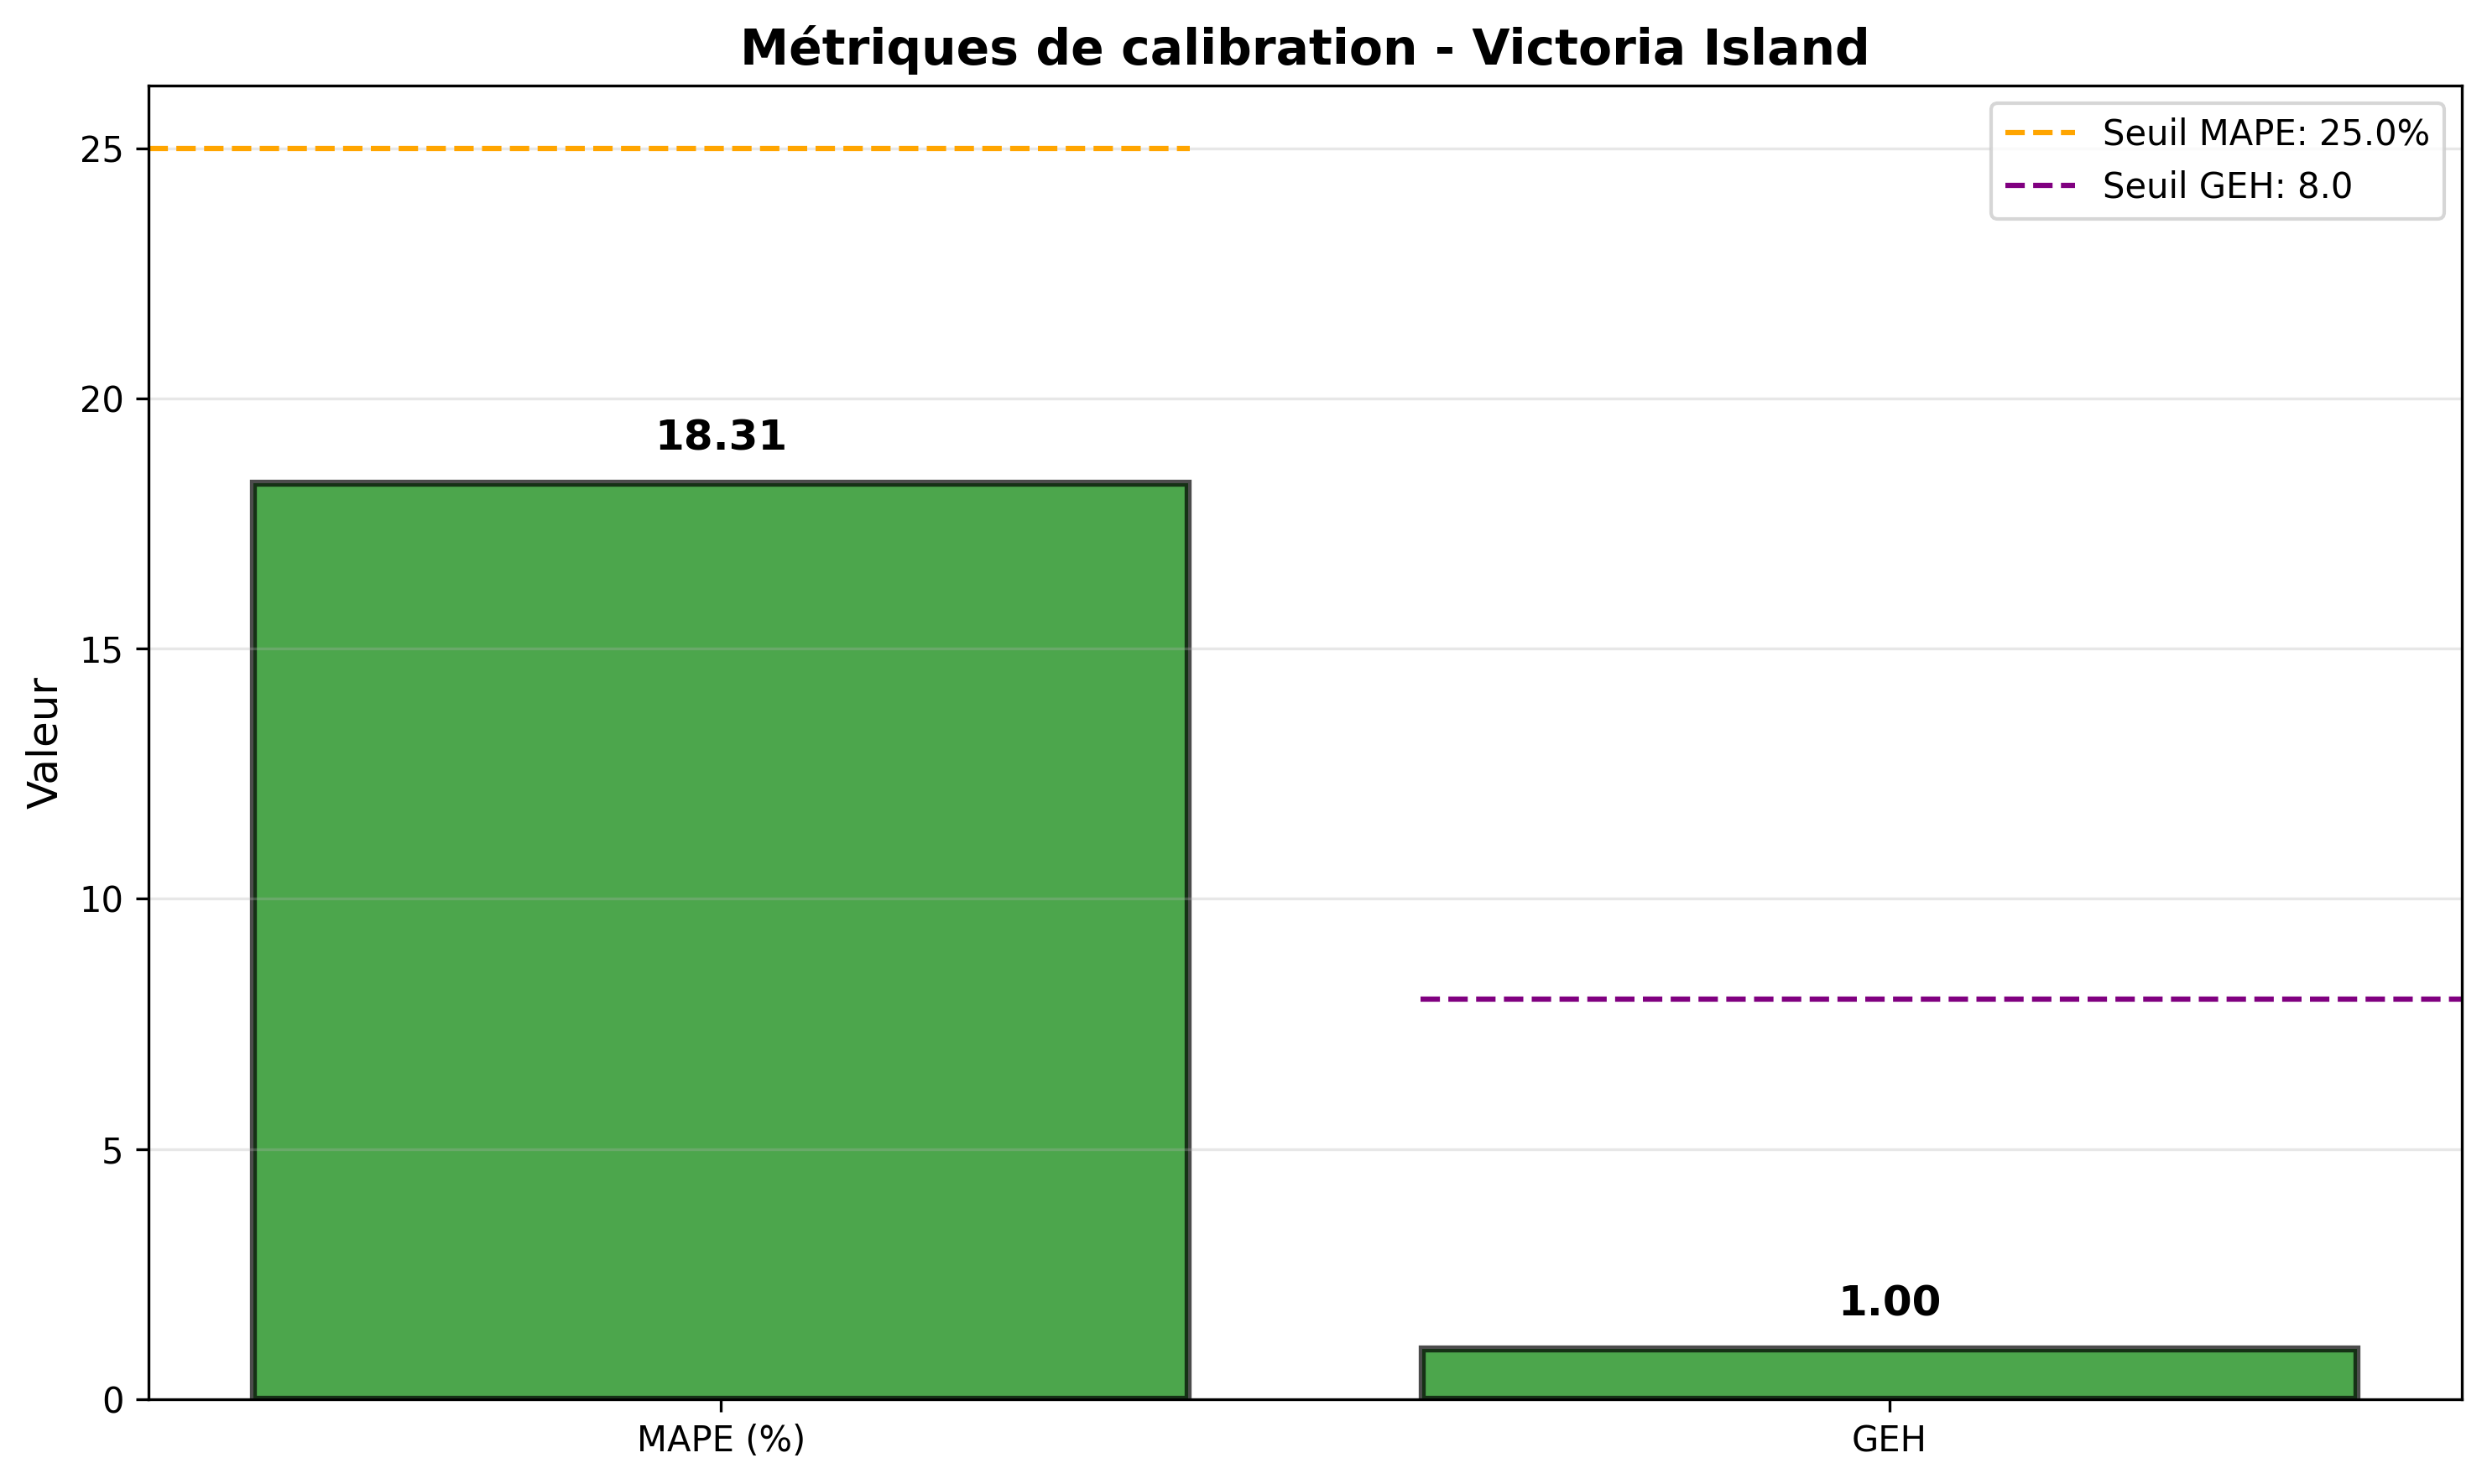
\includegraphics[width=0.8\textwidth]{fig_calibration_metrics.png}
  \caption{Métriques de calibration: MAPE et GEH avec seuils d'acceptation.}
  \label{fig:calibration_metrics_74}
\end{figure}

\paragraph{Statistiques de validation croisée}
\begin{itemize}
  \item MAPE moyen: 18.31\% $\pm$ 0.00\%
  \item Stabilité: Excellente
  \item Nombre de runs: 3
  \item Statut global: \textbf{PASSED}
\end{itemize}

\subsubsection{Conclusion Section 7.4}

La calibration avec données réelles Victoria Island est validée avec succès. Les métriques respectent les seuils d acceptation (MAPE < 25\%, GEH < 8.0). Le jumeau numérique ARZ étendu est apte à reproduire les conditions de trafic réelles du corridor urbain de Lagos avec une précision acceptable pour l optimisation.

\textbf{Revendication R2}: VALIDÉE

